
%%%%%%%%%%%%%%%%%%%%%%%%%%%%%%%%%%%%%%%%%%%%%%%%
% Appendix
%%%%%%%%%%%%%%%%%%%%%%%%%%%%%%%%%%%%%%%%%%%%%%%%

\clearpage
\section{실험 설정과 전체 정확도 분석}\label{app:setup}\label{app:ablation}

Table~\ref{tab:performance_full}은 본문 Table~\ref{tab:performance}에서 위치별 최고 성능만 요약해 제시한 결과를, Prefix, Infix, Suffix별 전체 정확도로 다시 펼쳐 보인다. Table~\ref{tab:token_count}는 각 모델--벤치마크 조합에서 사용한 RSP 토큰 수 $L$을 정리한 것으로, 후보 집합 $\{10, 15, 20\}$에서 선택했다. 모든 실험은 단일 NVIDIA A6000 40GB GPU에서 greedy decoding으로 수행했으며, 최대 생성 길이는 MATH-500과 GSM8K에서 3{,}072 토큰, AIME24에서 4{,}096 토큰으로 고정했다. 배치 크기는 모델별로 고정했다(LLaMA-3.1-8B-Instruct와 Qwen2.5-Math-7B 계열은 16, Qwen2.5-Math-1.5B 계열은 32).

\begin{table}[ht]
\centering
\caption{모델 설정, 주입 위치, 벤치마크별 정확도(\%). 괄호 안 값은 baseline 대비 변화량이다. \textbf{굵게}는 최고 성능, \underline{밑줄}은 각 모델--벤치마크 조합에서 두 번째 성능을 뜻한다.}
\label{tab:performance_full}
\footnotesize
\renewcommand{\arraystretch}{0.9}
\begin{tabular}{ll ccc}
\toprule
\textbf{Model} & \textbf{Mode} & \textbf{MATH-500} & \textbf{GSM8K} & \textbf{AIME24} \\
\midrule
\multicolumn{5}{l}{\textit{Instruct Models}} \\
\midrule
\multirow{4}{*}{LLaMA-3.1-8B-Instruct} & Baseline & \textbf{52.20} & 85.75 & \underline{6.67} \\
 & Prefix & 45.00 {\scriptsize($-$7.2)} & 76.35 {\scriptsize($-$9.4)} & 3.33 {\scriptsize($-$3.3)} \\
 & Infix & \underline{49.40} {\scriptsize($-$2.8)} & \underline{85.97} {\scriptsize(+0.2)} & \textbf{10.00} {\scriptsize(+3.3)} \\
 & Suffix & \underline{49.40} {\scriptsize($-$2.8)} & \textbf{86.73} {\scriptsize(+1.0)} & \textbf{10.00} {\scriptsize(+3.3)} \\
\midrule
\multirow{4}{*}{Qwen2.5-Math-7B-Instruct} & Baseline & 83.20 & 95.45 & \underline{13.33} \\
 & Prefix & 81.40 {\scriptsize($-$1.8)} & 94.92 {\scriptsize($-$0.5)} & \underline{13.33} {\scriptsize(+0.0)} \\
 & Infix & \textbf{84.20} {\scriptsize(+1.0)} & \underline{95.60} {\scriptsize(+0.2)} & \textbf{16.67} {\scriptsize(+3.3)} \\
 & Suffix & \underline{83.40} {\scriptsize(+0.2)} & \textbf{95.68} {\scriptsize(+0.2)} & \textbf{16.67} {\scriptsize(+3.3)} \\
\midrule
\multirow{4}{*}{Qwen2.5-Math-1.5B-Instruct} & Baseline & 73.00 & \underline{85.29} & 10.00 \\
 & Prefix & \underline{74.80} {\scriptsize(+1.8)} & \underline{85.29} {\scriptsize(+0.0)} & \underline{13.33} {\scriptsize(+3.3)} \\
 & Infix & \textbf{75.20} {\scriptsize(+2.2)} & \textbf{85.75} {\scriptsize(+0.5)} & 6.67 {\scriptsize($-$3.3)} \\
 & Suffix & 74.20 {\scriptsize(+1.2)} & 84.69 {\scriptsize($-$0.6)} & \textbf{20.00} {\scriptsize(+10.0)} \\
\midrule
\multicolumn{5}{l}{\textit{Base Models (Raw Text)}} \\
\midrule
\multirow{4}{*}{Qwen2.5-Math-7B} & Baseline & \textbf{72.20} & \underline{84.15} & 6.67 \\
 & Prefix & \underline{71.60} {\scriptsize($-$0.6)} & \textbf{84.31} {\scriptsize(+0.2)} & \textbf{16.67} {\scriptsize(+10.0)} \\
 & Infix & 63.20 {\scriptsize($-$9.0)} & 64.29 {\scriptsize($-$19.9)} & \textbf{16.67} {\scriptsize(+10.0)} \\
 & Suffix & 55.60 {\scriptsize($-$16.6)} & 54.13 {\scriptsize($-$30.0)} & \underline{13.33} {\scriptsize(+6.7)} \\
\midrule
\multirow{4}{*}{Qwen2.5-Math-1.5B} & Baseline & \underline{61.40} & \textbf{77.86} & \textbf{16.67} \\
 & Prefix & \textbf{64.40} {\scriptsize(+3.0)} & \underline{74.30} {\scriptsize($-$3.6)} & \underline{10.00} {\scriptsize($-$6.7)} \\
 & Infix & 63.20 {\scriptsize(+1.8)} & 73.92 {\scriptsize($-$3.9)} & \underline{10.00} {\scriptsize($-$6.7)} \\
 & Suffix & 54.60 {\scriptsize($-$6.8)} & 58.61 {\scriptsize($-$19.3)} & 3.33 {\scriptsize($-$13.3)} \\
\midrule
\multicolumn{5}{l}{\textit{Base Models + ChatML (Format Mismatch)}} \\
\midrule
\multirow{4}{*}{Qwen2.5-Math-7B} & Baseline & 52.20 & 58.30 & \textbf{23.33} \\
 & Prefix & 59.20 {\scriptsize(+7.0)} & 56.41 {\scriptsize($-$1.9)} & \underline{3.33} {\scriptsize($-$20.0)} \\
 & Infix & \underline{62.00} {\scriptsize(+9.8)} & \underline{69.07} {\scriptsize(+10.8)} & \textbf{23.33} {\scriptsize(+0.0)} \\
 & Suffix & \textbf{70.40} {\scriptsize(+18.2)} & \textbf{75.97} {\scriptsize(+17.7)} & \textbf{23.33} {\scriptsize(+0.0)} \\
\midrule
\multirow{4}{*}{Qwen2.5-Math-1.5B} & Baseline & 34.40 & 37.45 & \underline{13.33} \\
 & Prefix & \textbf{63.40} {\scriptsize(+29.0)} & \textbf{67.02} {\scriptsize(+29.6)} & \textbf{20.00} {\scriptsize(+6.7)} \\
 & Infix & 39.20 {\scriptsize(+4.8)} & 50.42 {\scriptsize(+13.0)} & 6.67 {\scriptsize($-$6.7)} \\
 & Suffix & \underline{51.00} {\scriptsize(+16.6)} & \underline{50.64} {\scriptsize(+13.2)} & \underline{13.33} {\scriptsize(+0.0)} \\
\bottomrule
\end{tabular}
\end{table}

\begin{table}[ht]
\centering
\caption{각 모델과 벤치마크에 사용한 RSP 토큰 수($L$).}
\label{tab:token_count}
\footnotesize
\renewcommand{\arraystretch}{0.9}
\begin{tabular}{lccc}
\toprule
\textbf{Model} & \textbf{MATH-500} & \textbf{GSM8K} & \textbf{AIME24} \\
\midrule
LLaMA-3.1-8B-Instruct & 15 & 20 & 15 \\
Qwen2.5-Math-7B-Instruct & 20 & 20 & 20 \\
Qwen2.5-Math-1.5B-Instruct & 20 & 10 & 20 \\
Qwen2.5-Math-7B & 10 & 10 & 20 \\
Qwen2.5-Math-1.5B & 10 & 10 & 20 \\
Qwen2.5-Math-1.5B (ChatML) & 20 & 20 & 10 \\
Qwen2.5-Math-7B (ChatML) & 20 & 20 & 20 \\
\bottomrule
\end{tabular}
\end{table}

% ================================================================
\subsection{RSP 주입 위치와 프롬프트 템플릿}\label{app:injection_positions}
% ================================================================

아래에는 모든 모델 유형에서 주입 위치별 프롬프트 구조를 정리했다. \textcolor{blue!70!black}{파란색 텍스트}는 RSP 임베딩, \textcolor{purple}{보라색 텍스트}는 특수 토큰을 뜻한다.

% --------------------------------
\subsubsection{Prefix}
% --------------------------------

Prefix 주입에서는 RSP 임베딩을 프롬프트 임베딩 앞에 연결한다. 텍스트 자체는 수정하지 않는다.

\paragraph{ChatML (Qwen Instruct / Base + ChatML).}
\begin{tcolorbox}[colback=gray!5, colframe=black!60, arc=3pt, boxrule=0.5pt, fontupper=\footnotesize\ttfamily, breakable]
\textcolor{blue!70!black}{[Random Embeddings ($L$ tokens)]}\\
\textcolor{purple}{<|im\_start|>}system\\
Please reason step by step, and put your final answer within \textbackslash boxed\{\}.\textcolor{purple}{<|im\_end|>}\\
\textcolor{purple}{<|im\_start|>}user\\
\{question\}\textcolor{purple}{<|im\_end|>}\\
\textcolor{purple}{<|im\_start|>}assistant
\end{tcolorbox}

\paragraph{LLaMA Chat Template.}
\begin{tcolorbox}[colback=gray!5, colframe=black!60, arc=3pt, boxrule=0.5pt, fontupper=\footnotesize\ttfamily, breakable]
\textcolor{blue!70!black}{[Random Embeddings ($L$ tokens)]}\\
\textcolor{purple}{<|begin\_of\_text|>}\\
\textcolor{purple}{<|start\_header\_id|>}system\textcolor{purple}{<|end\_header\_id|>}\\
Cutting Knowledge Date: December 2023\\
Today Date: 26 Jul 2024\\
Please reason step by step, and put your final answer within \textbackslash boxed\{\}.\textcolor{purple}{<|eot\_id|>}\\
\textcolor{purple}{<|start\_header\_id|>}user\textcolor{purple}{<|end\_header\_id|>}\\
\{question\}\textcolor{purple}{<|eot\_id|>}\\
\textcolor{purple}{<|start\_header\_id|>}assistant\textcolor{purple}{<|end\_header\_id|>}
\end{tcolorbox}

\paragraph{Raw Text (Qwen Base).}
\begin{tcolorbox}[colback=gray!5, colframe=black!60, arc=3pt, boxrule=0.5pt, fontupper=\footnotesize\ttfamily, breakable]
\textcolor{blue!70!black}{[Random Embeddings ($L$ tokens)]}\\
\{question\}\\
Please reason step by step, and put your final answer within \textbackslash boxed\{\}.
\end{tcolorbox}

% --------------------------------
\subsubsection{Infix}
% --------------------------------

Infix 주입에서는 설명 문구와 특수 토큰을 프롬프트 내부에 넣은 뒤, 그 특수 토큰 위치를 임베딩 수준에서 RSP로 교체한다.

\paragraph{ChatML (Qwen Instruct / Base + ChatML).}
\begin{tcolorbox}[colback=gray!5, colframe=black!60, arc=3pt, boxrule=0.5pt, fontupper=\footnotesize\ttfamily, breakable]
\textcolor{purple}{<|im\_start|>}system\\
Please reason step by step, and put your final answer within \textbackslash boxed\{\}.\textcolor{purple}{<|im\_end|>}\\
\textcolor{purple}{<|im\_start|>}user\\
\{question\}\\[0.3em]
\textcolor{gray}{There are \{$L$\} special tokens that contain compressed latent reasoning information that might be useful for your reasoning. If these tokens are useful for your case, you can use them as reference. If these tokens are not useful for your case, you can ignore them and focus back to solving the problem.}\\[0.3em]
Here are the \{$L$\} special tokens: \textcolor{blue!70!black}{<special\_token\_1>...<special\_token\_$L$>}\\
\textcolor{purple}{<|im\_end|>}\\
\textcolor{purple}{<|im\_start|>}assistant
\end{tcolorbox}

\paragraph{LLaMA Chat Template.}
\begin{tcolorbox}[colback=gray!5, colframe=black!60, arc=3pt, boxrule=0.5pt, fontupper=\footnotesize\ttfamily, breakable]
\textcolor{purple}{<|begin\_of\_text|>}\\
\textcolor{purple}{<|start\_header\_id|>}system\textcolor{purple}{<|end\_header\_id|>}\\
Cutting Knowledge Date: December 2023\\
Today Date: 26 Jul 2024\\
Please reason step by step, and put your final answer within \textbackslash boxed\{\}.\textcolor{purple}{<|eot\_id|>}\\
\textcolor{purple}{<|start\_header\_id|>}user\textcolor{purple}{<|end\_header\_id|>}\\
\{question\}\\[0.3em]
\textcolor{gray}{There are \{$L$\} special tokens that contain compressed latent reasoning information that might be useful for your reasoning. If these tokens are useful for your case, you can use them as reference. If these tokens are not useful for your case, you can ignore them and focus back to solving the problem.}\\[0.3em]
Here are the \{$L$\} special tokens:\\
\textcolor{blue!70!black}{<reserved\_special\_token\_0>...}\\
\textcolor{blue!70!black}{<reserved\_special\_token\_$L$>}\\
\textcolor{purple}{<|eot\_id|>}\\
\textcolor{purple}{<|start\_header\_id|>}assistant\textcolor{purple}{<|end\_header\_id|>}
\end{tcolorbox}

\paragraph{Raw Text (Qwen Base).}
\begin{tcolorbox}[colback=gray!5, colframe=black!60, arc=3pt, boxrule=0.5pt, fontupper=\footnotesize\ttfamily, breakable]
\{question\}\\[0.3em]
\textcolor{gray}{There are \{$L$\} special tokens that contain compressed latent reasoning information that might be useful for your reasoning. If these tokens are useful for your case, you can use them as reference. If these tokens are not useful for your case, you can ignore them and focus back to solving the problem.}\\[0.3em]
Here are the \{$L$\} special tokens: \textcolor{blue!70!black}{<special\_token\_1>...<special\_token\_$L$>}\\[0.3em]
Please reason step by step, and put your final answer within \textbackslash boxed\{\}.
\end{tcolorbox}

% --------------------------------
\subsubsection{Suffix}
% --------------------------------

채팅 템플릿 모델에서는 end-of-turn 토큰 바로 앞에 RSP 임베딩을 넣고, raw text 모델에서는 프롬프트 마지막에 RSP 임베딩을 이어 붙인다.

\paragraph{ChatML (Qwen Instruct / Base + ChatML).}
\begin{tcolorbox}[colback=gray!5, colframe=black!60, arc=3pt, boxrule=0.5pt, fontupper=\footnotesize\ttfamily, breakable]
\textcolor{purple}{<|im\_start|>}system\\
Please reason step by step, and put your final answer within \textbackslash boxed\{\}.\textcolor{purple}{<|im\_end|>}\\
\textcolor{purple}{<|im\_start|>}user\\
\{question\}\textcolor{blue!70!black}{[Random Embeddings ($L$ tokens)]}\textcolor{purple}{<|im\_end|>}\\
\textcolor{purple}{<|im\_start|>}assistant
\end{tcolorbox}

\paragraph{LLaMA Chat Template.}
\begin{tcolorbox}[colback=gray!5, colframe=black!60, arc=3pt, boxrule=0.5pt, fontupper=\footnotesize\ttfamily, breakable]
\textcolor{purple}{<|begin\_of\_text|>}\\
\textcolor{purple}{<|start\_header\_id|>}system\textcolor{purple}{<|end\_header\_id|>}\\
Cutting Knowledge Date: December 2023\\
Today Date: 26 Jul 2024\\
Please reason step by step, and put your final answer within \textbackslash boxed\{\}.\textcolor{purple}{<|eot\_id|>}\\
\textcolor{purple}{<|start\_header\_id|>}user\textcolor{purple}{<|end\_header\_id|>}\\
\{question\}\textcolor{blue!70!black}{[Random Embeddings ($L$ tokens)]}\textcolor{purple}{<|eot\_id|>}\\
\textcolor{purple}{<|start\_header\_id|>}assistant\textcolor{purple}{<|end\_header\_id|>}
\end{tcolorbox}

\paragraph{Raw Text (Qwen Base).}
\begin{tcolorbox}[colback=gray!5, colframe=black!60, arc=3pt, boxrule=0.5pt, fontupper=\footnotesize\ttfamily, breakable]
\{question\}\\
Please reason step by step, and put your final answer within \textbackslash boxed\{\}.\textcolor{blue!70!black}{[Random Embeddings ($L$ tokens)]}
\end{tcolorbox}

% ================================================================
\subsection{정답 추출과 채점}
% ================================================================

최종 정답은 fallback 체인을 통해 모델 출력에서 추출한다. 각 단계는 순서대로 시도하며, 추출에 실패하면 다음 단계로 넘어간다.

\begin{tcolorbox}[colback=gray!5, colframe=black!60, arc=3pt, boxrule=0.5pt, title=\textbf{정답 추출 fallback 체인}, fonttitle=\small, coltitle=black, colbacktitle=gray!20]
\small
\begin{enumerate}[leftmargin=*, nosep]
  \item \texttt{"final answer is \$...\$. I hope"} 패턴(Minerva 형식)
  \item \texttt{\textbackslash boxed\{...\}}: 마지막 비어 있지 않은 box를 사용하고, 빈 \texttt{\textbackslash boxed\{\}}는 건너뜀
  \item \texttt{"the answer is"} 뒤 텍스트
  \item \texttt{"final answer is"} 뒤 텍스트
  \item 출력 마지막 숫자(regex fallback)
\end{enumerate}
\end{tcolorbox}

\vspace{0.5em}
추출된 정답은 \texttt{\$}, \texttt{\textbackslash left}, \texttt{\textbackslash right}, 단위 문자열을 제거해 정규화한다. 채점은 symbolic equivalence checking으로 수행하며, 정확한 문자열 일치, 수치 비교(\texttt{math.isclose}, \texttt{rel\_tol=1e-4}), SymPy symbolic simplification을 차례로 적용한다.

% ================================================================
\subsection{재현한 선행연구의 하이퍼파라미터}
% ================================================================

모든 선행 방법은 Qwen2.5-Math-1.5B-Instruct와 Qwen2.5-Math-7B-Instruct에서 재현했으며, greedy decoding(temperature $= 0$)과 통일된 answer extraction pipeline으로 평가했다.

\paragraph{TTSV.} Prefix 길이는 20이며, AdamW optimizer로 20 epoch 동안 학습했다. 배치 크기는 2, gradient accumulation은 8 step, 스케줄은 선형 learning rate schedule을 사용했다. Learning rate는 Qwen-1.5B에 1e-3, Qwen-7B에 1e-5를 사용했다.

\paragraph{LTPO.} Table~\ref{tab:hp_ltpo}는 벤치마크별 하이퍼파라미터를 정리한 것이다.

\begin{table}[ht]
\centering
\caption{LTPO 하이퍼파라미터.}
\label{tab:hp_ltpo}
\footnotesize
\renewcommand{\arraystretch}{0.9}
\begin{tabular}{lccc}
\toprule
\textbf{Parameter} & \textbf{GSM8K} & \textbf{MATH-500} & \textbf{AIME24} \\
\midrule
tokens & 8 & 8 & 8 \\
steps & 20 & 20 & 20 \\
top\_k & 10 & 10 & 10 \\
sigma & 20 & 20 & 5 \\
sigma\_decay & 0.95 & 0.95 & 0.95 \\
lr & 1e-2 & 5e-3 & 5e-2 \\
\bottomrule
\end{tabular}
\end{table}

\paragraph{SoftCoT.} Projection module은 10 epoch 동안 학습했다. Thought token 수는 학습 시 32, 평가 시 4다. 배치 크기는 GSM8K에서 4, MATH에서는 1이며 gradient accumulation 4를 사용했다. 작은 모델(assistant)은 두 설정 모두 Qwen2.5-Math-1.5B-Instruct이고, 큰 모델은 Qwen2.5-Math-1.5B-Instruct(learning rate 2e-5) 또는 Qwen2.5-Math-7B-Instruct(learning rate 5e-6)이다. MATH-500과 AIME24 평가는 GSM8K에서 학습한 projection module을 사용했는데, MATH에서 학습한 버전보다 더 높은 정확도를 보였기 때문이다.

% ================================================================
\subsection{전체 엔트로피 곡선}
% ================================================================

Figure~\ref{fig:app_full_entropy}는 entropy, top-1 probability, varentropy의 전체 정규화 생성 궤적(0--100\%)을 보여준다. 모든 방법은 생성 초반 단계를 지나면 비슷한 수준으로 수렴하며, 이는 RSP가 유도하는 분포 변화가 초기 추론 단계에 국소화되어 있음을 다시 확인해 준다.

\begin{figure}[ht]
  \centering
  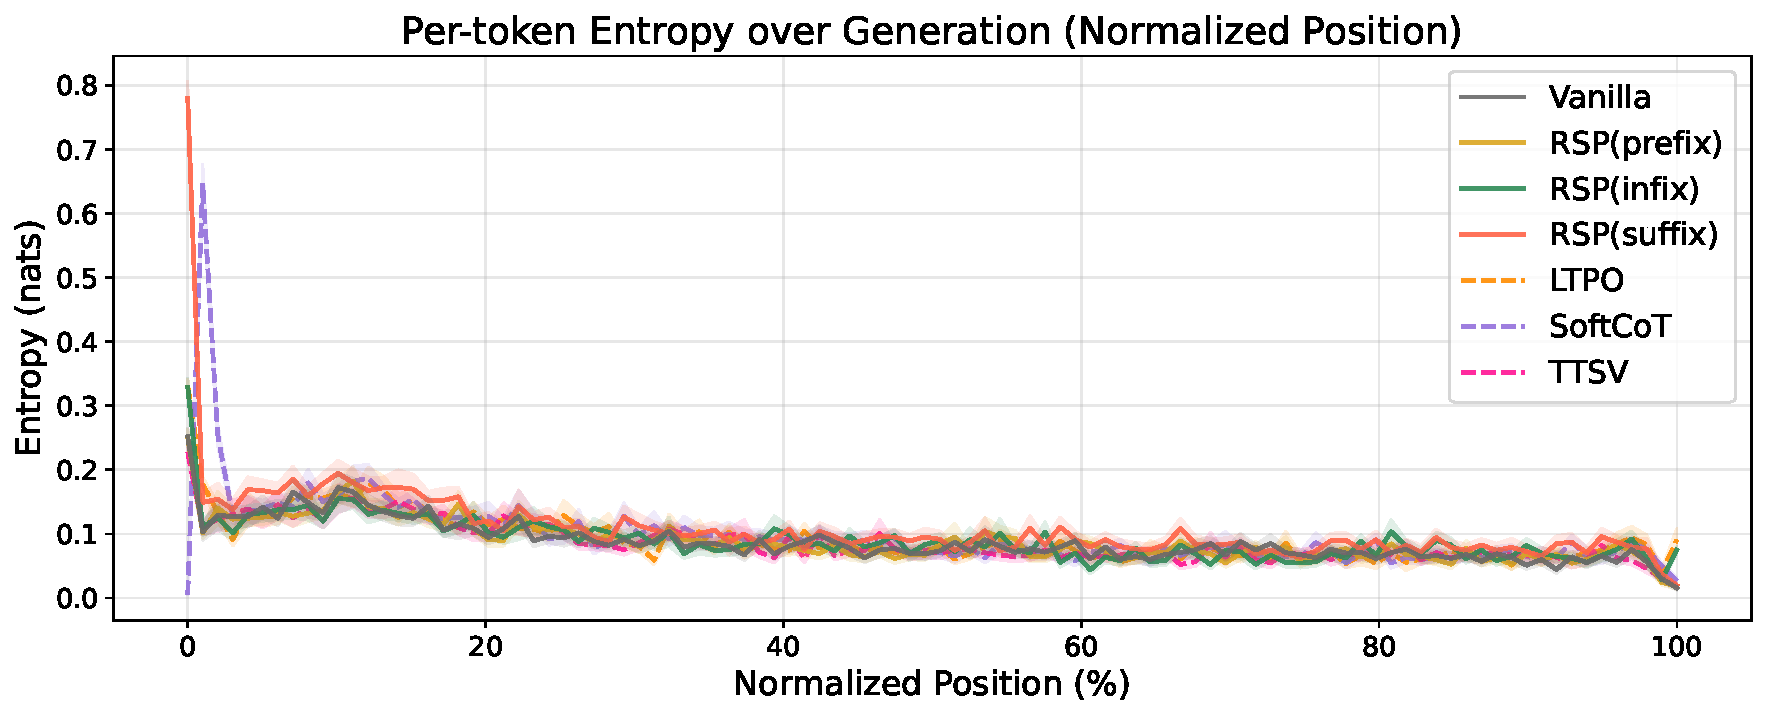
\includegraphics[width=0.85\textwidth]{img/entropy/full_entropy.pdf}\\[0.4em]
  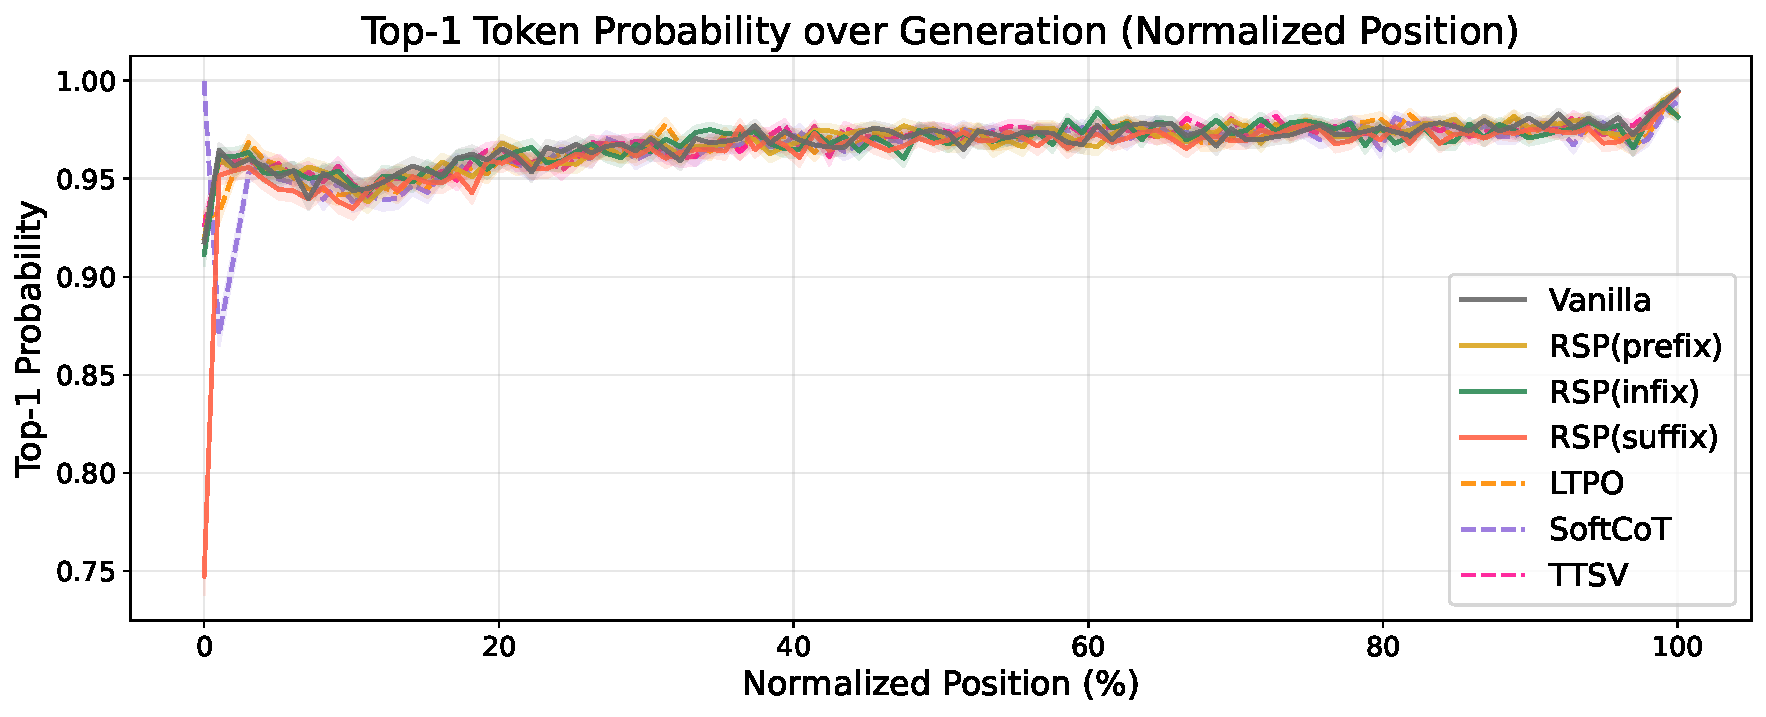
\includegraphics[width=0.85\textwidth]{img/entropy/full_top1prob.pdf}\\[0.4em]
  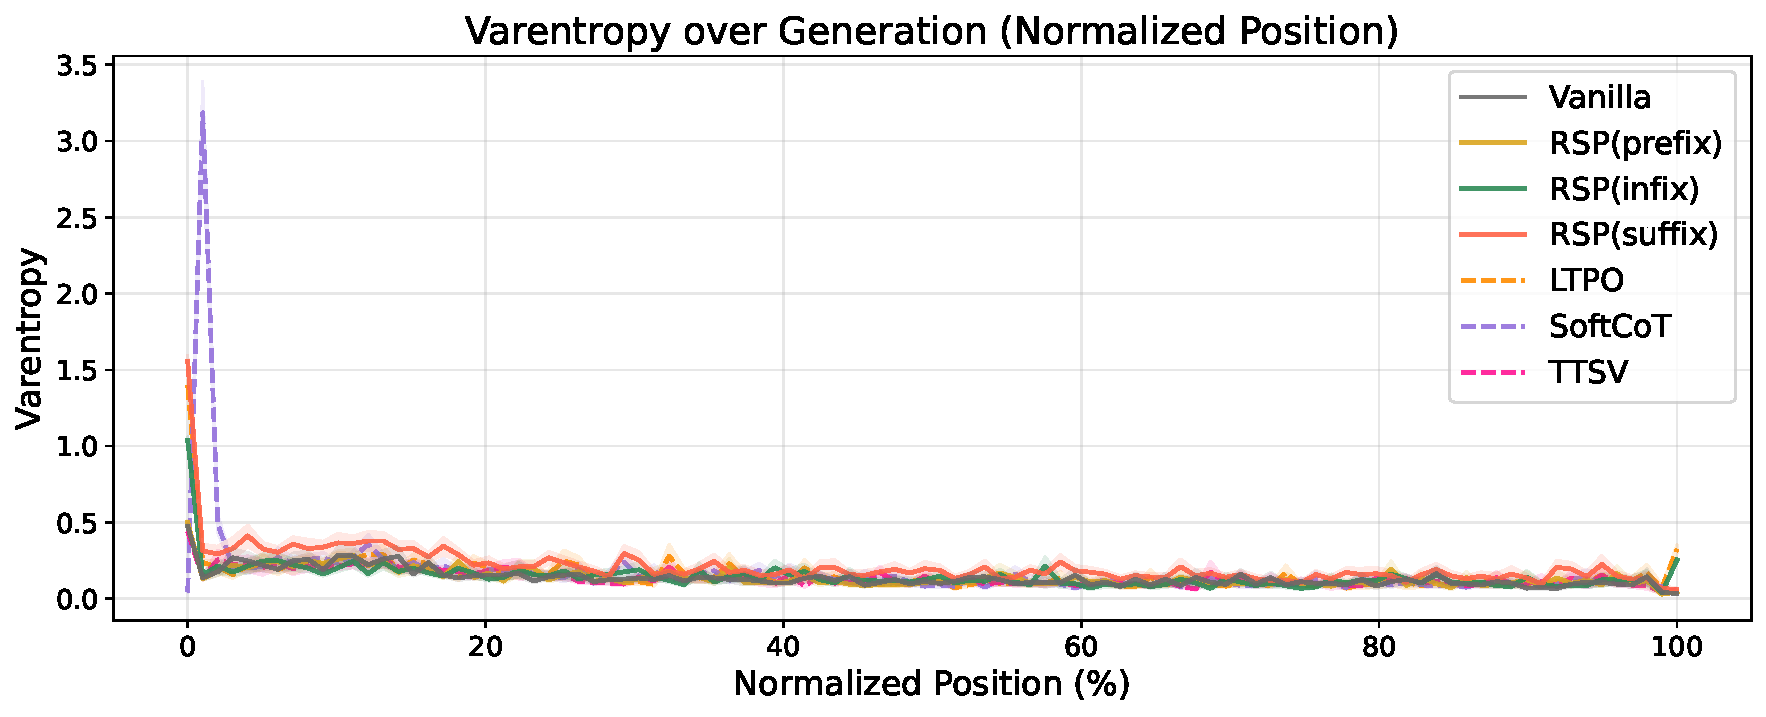
\includegraphics[width=0.85\textwidth]{img/entropy/full_varentropy.pdf}
  \caption{전체 정규화 생성 궤적(0--100\%)에서의 평균 entropy(위), top-1 probability(가운데), varentropy(아래). MATH-500 전체 평균이며, 음영은 $\pm$1 SEM을 뜻한다. 실선은 RSP 변형과 baseline, 점선은 기존 soft prompt 방법이다. 모든 방법은 초반 단계를 지나면 수렴한다.}
  \label{fig:app_full_entropy}
\end{figure}

\clearpage
\section{의미적 다양성에 대한 추가 분석}\label{app:semantic}

이 부록은 Section~\ref{sec:diversity}에서 보고한 의미적 다양성 결과를 보충한다. 더 넓은 문제 집합에 대해 문제별 t-SNE 도표를 함께 제시한다.

\begin{figure}[ht]
  \centering
  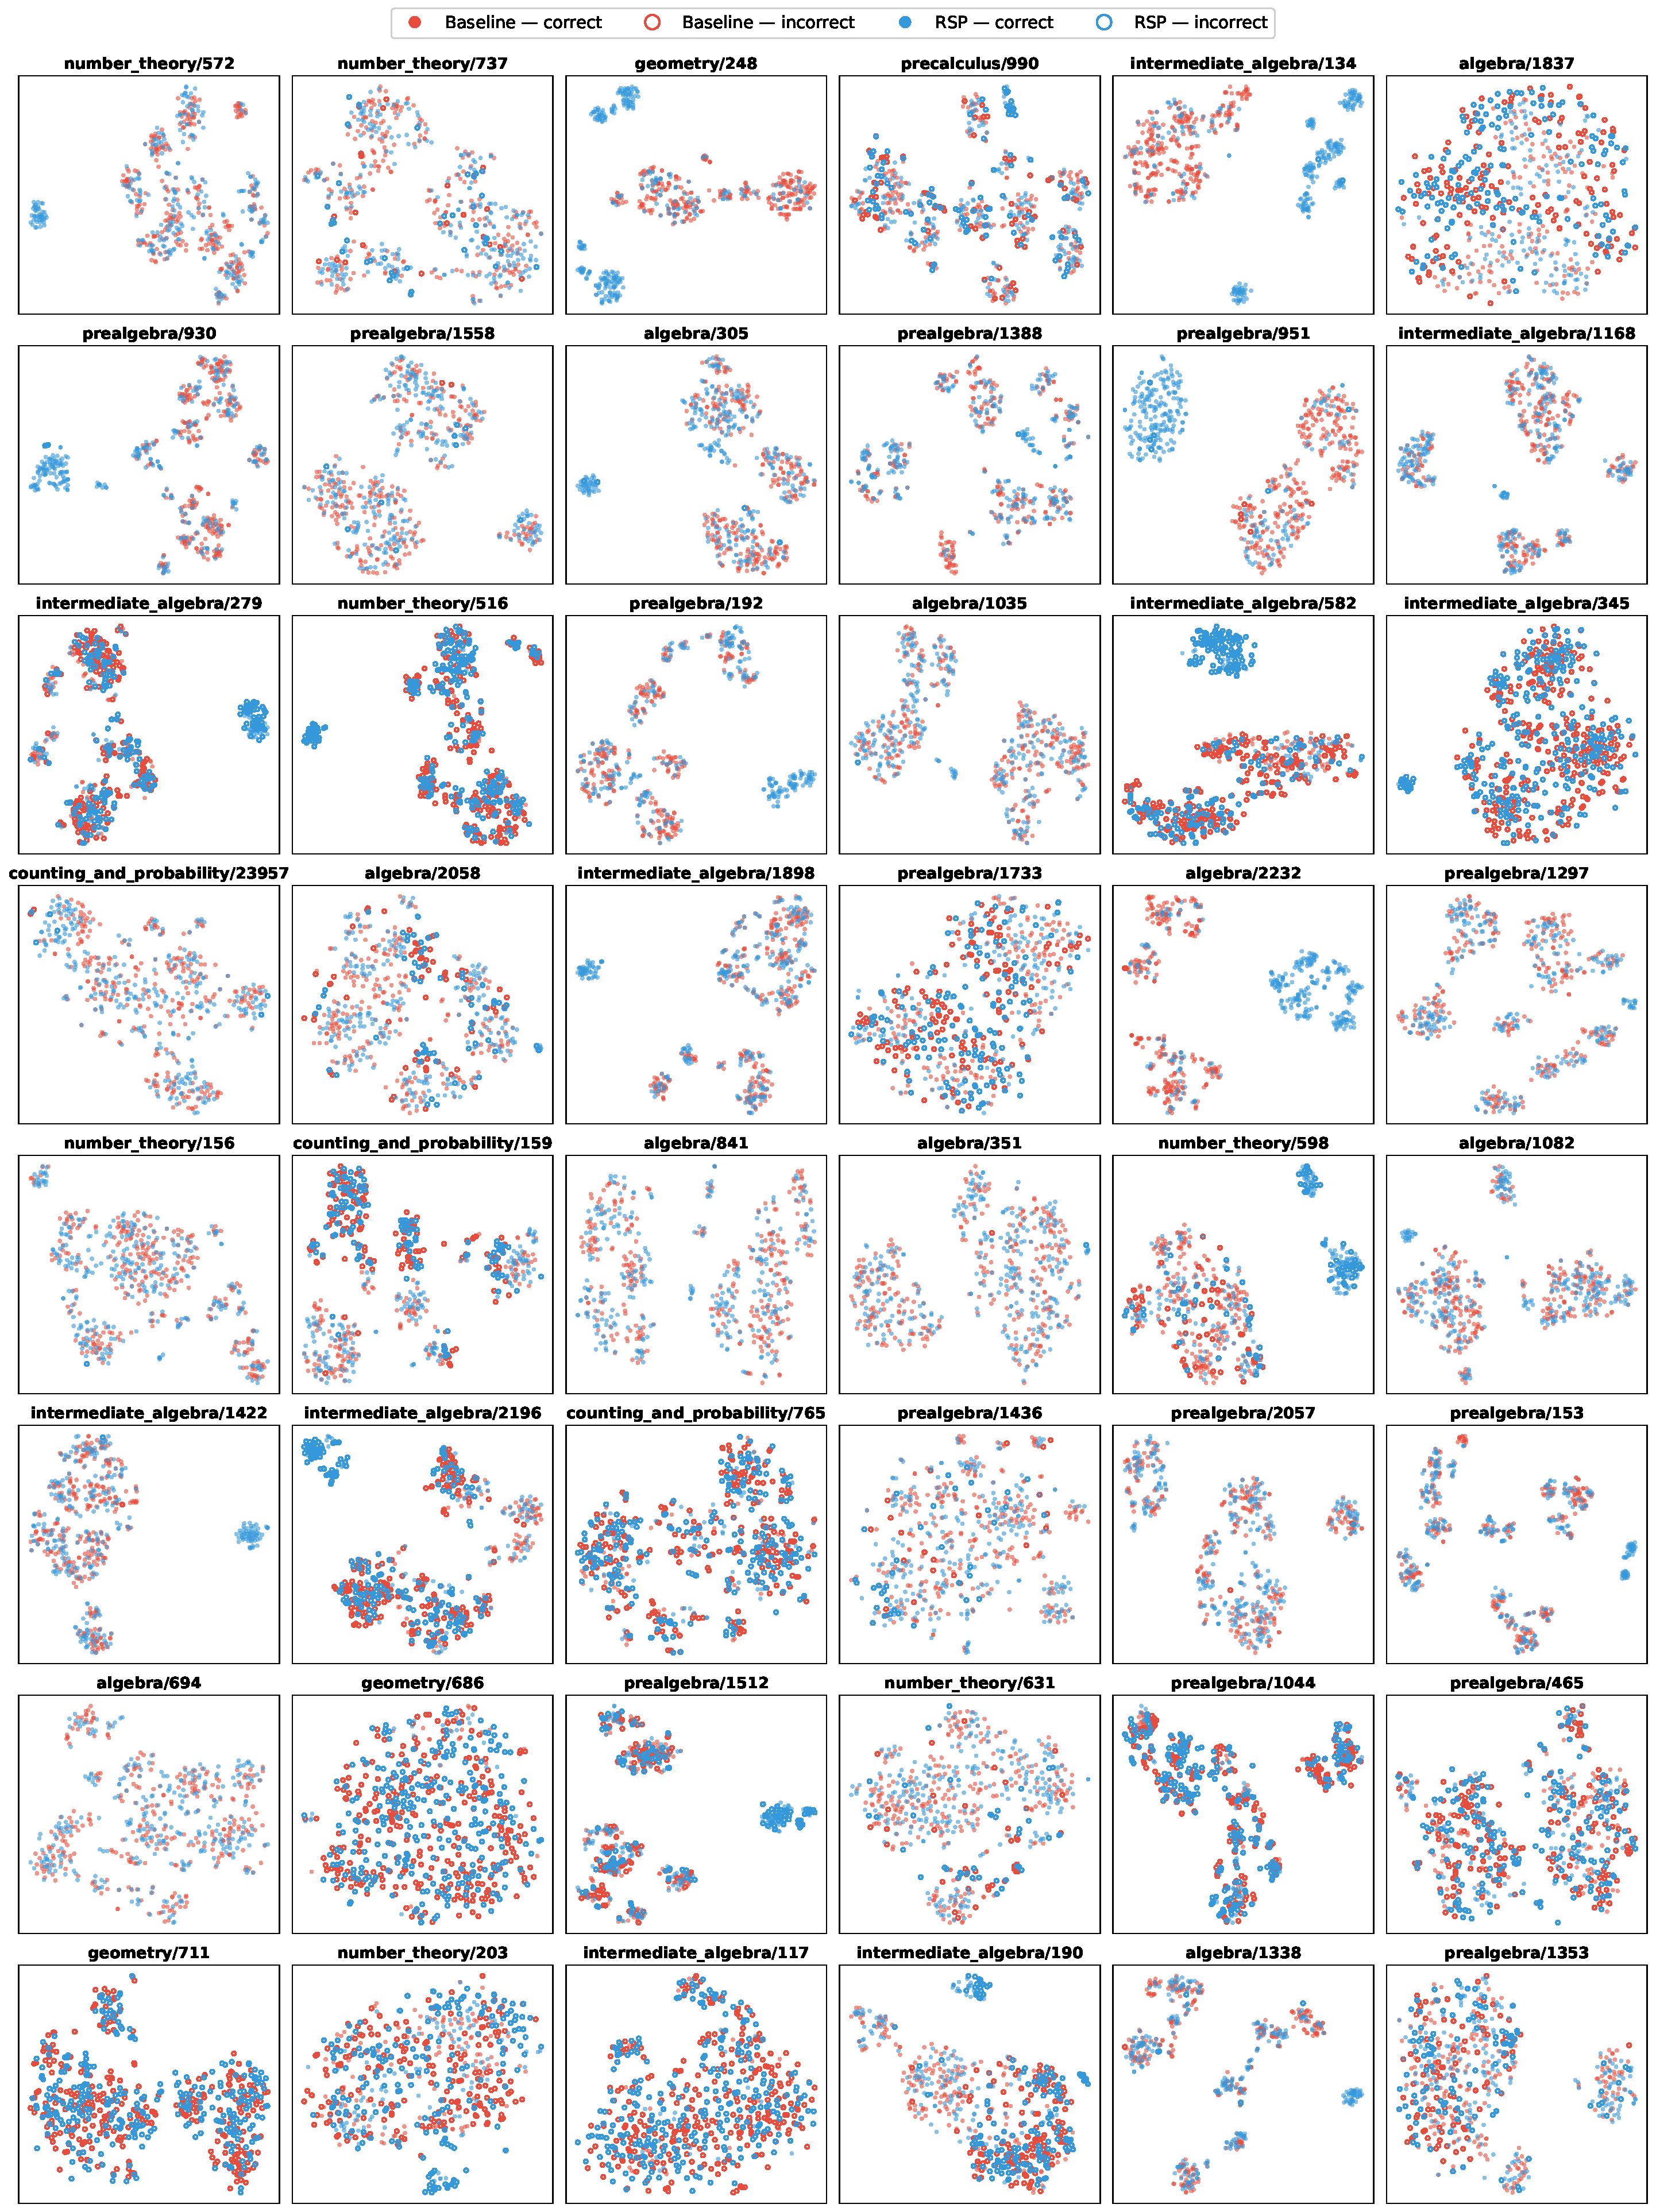
\includegraphics[width=\textwidth,height=0.75\textheight,keepaspectratio]{img/diversity/appendix_tsne_grid.pdf}
  \caption{평가한 64개 MATH-500 문제 중 48개에 대한 BGE-M3 임베딩의 t-SNE 투영(6$\times$8 격자). 각 subplot은 Qwen2.5-Math-1.5B-Instruct에서 $\tau=1.0$으로 생성한 baseline 300개(빨강)와 RSP suffix 300개(파랑)를 보여준다. 채워진 표식은 정답, 빈 표식은 오답이며, 제목은 \texttt{subject/problem\_id}를 뜻한다. 대부분의 문제에서 RSP 궤적은 여러 개의 분리된 영역으로 퍼지는 반면, baseline 샘플은 하나의 지배적 클러스터에 더 집중된다.}
  \label{fig:app_tsne_grid}
\end{figure}

\clearpage
\section{토큰 수준 분포 지표}\label{app:token_metrics}

이 부록은 Section~\ref{sec:diversity}의 토큰 수준 분석에 사용한 세 지표를 형식적으로 정의한다. $P_{\text{base}}$는 $\tau=1.0$에서의 baseline 다음 토큰 분포, $P_{\text{target}}$은 비교 대상 분포(예: $\tau=2.0$의 baseline, 또는 $\tau=1.0$의 RSP)라 하자. 모든 지표는 첫 생성 단계에서 저장한 logits로부터 해석적으로 계산한다.

\paragraph{Spearman 순위 상관.}
Spearman의 $\rho$는 두 분포의 토큰 순위 사이 Pearson 상관계수다.
\begin{equation}
\rho \;=\; \mathrm{Pearson}\!\left(\mathrm{rank}(P_{\text{target}}),\; \mathrm{rank}(P_{\text{base}})\right).
\end{equation}
Temperature scaling $P^{(\tau)} \propto P^{1/\tau}$는 엄격한 단조 변환이므로, 어떤 $\tau > 0$에서도 토큰 순서를 정확히 보존한다. 따라서 $\rho = 1$은 수학적 항등식이다. 그러므로 $\rho < 1$은 temperature scaling만으로는 만들 수 없는 순위 재조직이 일어났음을 뜻한다.

\paragraph{Top-$K$ 밖의 질량.}
$\mathrm{TopK}(P_{\text{base}})$를 $P_{\text{base}}$에서 확률이 가장 높은 $K$개 토큰의 집합이라 하자. 비교 대상 분포가 이 집합 \emph{밖에} 두는 확률 질량은
\begin{equation}
\mathrm{MassOutside}_K \;=\; 1 - \sum_{t \in \mathrm{TopK}(P_{\text{base}})} P_{\text{target}}(t).
\end{equation}
이 지표는 지지 집합 확장을 직접 측정한다. 즉 baseline의 선호 집합에 없던 토큰에 비교 대상이 얼마나 많은 확률을 배정하는지를 본다. 본문에 보고한 값은 $K = 10$을 사용했다.

\paragraph{Jensen--Shannon divergence.}
Kullback--Leibler divergence의 대칭적이고 bounded된 형태는 다음과 같다.
\begin{equation}
\mathrm{JS}(P, Q) \;=\; \tfrac{1}{2}\,\mathrm{KL}(P \,\|\, M) + \tfrac{1}{2}\,\mathrm{KL}(Q \,\|\, M), \qquad M = \tfrac{1}{2}(P + Q).
\end{equation}
로그는 밑이 2이므로 $\mathrm{JS} \in [0, 1]$이다. 저장한 top-100 바깥의 토큰에는 softmax 전에 sentinel logit($-10^9$)을 넣었는데, 본 설정에서는 top-5가 이미 확률 질량의 $99.9\%$ 이상을 덮기 때문에 이 근사는 무시 가능하다.

\clearpage
\section{무작위 프롬프트는 왜 의미적으로 중립적이고 방향적으로 포괄적인가}\label{app:why_random}

이 부록은 Section~\ref{sec:multipath}에서 사용한 주장을 형식화한다. 핵심은 무작위 프롬프트가 유용한 잠재 의미를 담고 있다는 것이 아니다. 더 약하고 정확한 주장은, 중심화한 뒤에는 어떤 미리 정한 의미 방향도 체계적으로 편들지 않으면서도, 고정된 분산 예산 아래 모든 방향을 덮을 수 있다는 것이다. 이는 언어학적 의미가 완전히 사라진다는 주장이 아니라, 섭동 방향의 기하학적 성질에 관한 명제다.

\subsection{의미적 중립성}

$\bar{h} \sim \mathcal{N}(0, \sigma^2 \mathbf{I}_d)$라 하고, $\bar{h}\neq 0$일 때 $\hat{h} := \bar{h}/\|\bar{h}\|$라 하자. 또한 $u_1,\dots,u_M \in \mathbb{S}^{d-1}$를 의미 anchor 방향을 나타내는 임의의 고정 단위벡터라 하자.

\begin{lemma}[의미적 중립성]\label{lem:semantic_neutrality_proof}\label{lem:semantic_neutrality}
보편 상수 $C$가 존재하여, 모든 $\delta \in (0,1)$에 대해
\[
\Pr\!\left[
\max_{r \in [M]} |\hat{h}^{\top} u_r|
\le
C \sqrt{\frac{\log(M/\delta)}{d}}
\right]
\ge 1-\delta.
\]
즉 등방성 가우시안 프롬프트의 정규화된 방향은, 고정된 유한 개의 의미 anchor 전체에 대해 높은 확률로 거의 직교한다.
\end{lemma}

\begin{proof}
각 고정 $u_r$에 대해 회전 불변성으로부터 $u_r^\top \bar{h} \sim \mathcal{N}(0,\sigma^2)$가 성립하므로,
\[
\Pr\big(|u_r^\top \bar{h}| \ge t\big) \le 2\exp\!\left(-\frac{t^2}{2\sigma^2}\right).
\]
$r \in [M]$ 전체에 대해 union bound를 적용하면
\[
\Pr\!\left[\max_{r \in [M]} |u_r^\top \bar{h}| \ge t\right]
\le
2M \exp\!\left(-\frac{t^2}{2\sigma^2}\right).
\]
한편 표준 chi-square concentration으로부터 보편 상수 $c>0$가 존재하여
\[
\Pr\!\left[\|\bar{h}\| \le \frac{\sigma \sqrt{d}}{2}\right]
\le
\exp(-cd)
\]
가 성립한다. 사건 $\|\bar{h}\| \ge \sigma\sqrt{d}/2$ 위에서는
\[
|\hat{h}^{\top} u_r|
=
\frac{|u_r^\top \bar{h}|}{\|\bar{h}\|}
\le
\frac{2 |u_r^\top \bar{h}|}{\sigma \sqrt{d}}.
\]
이제
\[
t = C' \sigma \sqrt{\log(M/\delta)}
\]
로 두고 $C'$를 충분히 큰 상수로 잡으면, 두 bound를 결합해
\[
\max_{r \in [M]} |\hat{h}^{\top} u_r|
\le
C \sqrt{\frac{\log(M/\delta)}{d}}
\]
가 적어도 $1-\delta$ 확률로 성립한다.
\end{proof}

토큰 임베딩과의 대비는 즉각적이다. $e_s \neq 0$를 고정된 토큰 임베딩이라 하고 $\hat{e}_s := e_s/\|e_s\|$라 하자. 이때 anchor 방향을 $u = \hat{e}_s$로 잡으면
\[
|\hat{e}_s^\top u| = 1.
\]
즉 토큰 프롬프트는 적어도 하나의 의미 방향과 최대 정렬을 이루지만, 등방성 무작위 프롬프트는 어떤 고정된 유한 집합의 의미 방향에도 거의 직교한다. 우리가 말하는 ``의미적 비개입성''은 바로 이 뜻이다. 토큰은 의미적 commitment를 주입하는 반면, 무작위 프롬프트는 의미적으로 특정 방향에 묶이지 않은 섭동으로 기능한다.

\subsection{Theorem~\ref{thm:minimax_directional_coverage} (미니맥스 방향 커버리지)의 증명}

본문에서 사용한 local linear logit surrogate에 직접 등장하는 양은 단위벡터 $b$에 대해 $b$ 방향의 1차 섭동 에너지 $\mathrm{Var}_{h\sim D}(b^\top h)=b^\top\Sigma_D b$이다. $\min_{\|b\|=1}b^\top\Sigma_D b = \lambda_{\min}(\Sigma_D)$이므로 최소 방향 분산은 정확히 $\lambda_{\min}(\Sigma_D)$이다.

\begin{proof}[Theorem~\ref{thm:minimax_directional_coverage}의 증명]
$\Sigma_D$의 고윳값을 $\lambda_1,\dots,\lambda_d$라 하면,
\[
\lambda_{\min}(\Sigma_D)
\le
\frac{1}{d}\sum_{m=1}^{d}\lambda_m
=
\frac{\mathrm{tr}(\Sigma_D)}{d}
\le
\frac{\rho^2}{d}.
\]
모든 고윳값이 같을 때, 즉 $\Sigma_D = (\rho^2/d)\mathbf{I}_d$일 때 그리고 그럴 때만 등호가 성립한다.
\end{proof}

이 정리는 등방성 무작위성의 장점을 형식화한다. RSP는 어떤 logit-sensitive 방향을 섭동해야 하는지 사전에 알지 못하므로, 고정된 분산 예산 아래에서 등방성 분포는 모든 방향에 대한 최악 경우 섭동량을 유일하게 최대화한다. 고정 토큰 프롬프트는 결정적 섭동이므로 $\Sigma_D=0$이고 $\lambda_{\min}=0$이며, 비등방 섭동은 항상 $\lambda_{\min}(\Sigma_D)<\rho^2/d$이므로 적어도 한 방향에서 등방 최적해보다 덜 탐색하게 된다.

\clearpage
\section{본문 이론 결과의 증명}\label{app:proofs}

% [본문 문단 5 메커니즘 1에 대한 증명]
% RSP perturbation term의 expectation, covariance, bias-to-variance ratio
\subsection{RSP가 유도하는 섭동의 성질}\label{app:rsp_noise}

본문 Eq.~\eqref{eq:decomp}의 분해 $\mathbf{x}_i^{(\ell+1)} = (1-w_{r,i}^{(\ell)})\tilde{\mathbf{x}}_i^{(\ell+1)} + \boldsymbol{\eta}_i^{(\ell)}$에서 무작위 기여 항 $\boldsymbol{\eta}_i^{(\ell)} = \sum_{j=1}^{L}\alpha_{i,n+j}^{(\ell)}\mathbf{v}_{r_j}^{(\ell)}$의 통계적 성질을 분석한다. 입력층의 RSP는 등방 가우시안이지만, layer $\ell$에서의 value vector $\mathbf{v}_{r_j}^{(\ell)}$는 attention, residual, LayerNorm, FFN, value projection을 차례로 통과한 결과이므로 일반적으로 등방 가우시안이 아니다. 따라서 layer 이후의 분석은 \emph{bounded second moment}만 가정한 형태로 약화하는 것이 안전하다.

\paragraph{조건부 기댓값과 상계.}
입력층 statistics에 의해 layer-별 mean·norm을
\[
m_v^{(\ell)} := \max_j \big\|\mathbb{E}[\mathbf{v}_{r_j}^{(\ell)}]\big\|,
\qquad
M_v^{(\ell)} := \max_j \mathbb{E}\big\|\mathbf{v}_{r_j}^{(\ell)}\big\|^2 \;<\; \infty
\]
라 두자(유한성은 implementation-side 가정으로 자연스럽다). 어텐션 가중치에 조건부로 두면
\begin{equation}
\bigl\|\mathbb{E}\!\left[\boldsymbol{\eta}_i^{(\ell)} \mid \alpha^{(\ell)}\right]\bigr\| \;\le\; w_{r,i}^{(\ell)} \, m_v^{(\ell)}.
\end{equation}
입력층($\ell=0$)에서는 등방 RSP에 대해 $m_v^{(0)} = |\mu_E|$이며, 항별 평균이 0에 가까운 임베딩 행렬에서 작아진다 — Table~\ref{tab:embed_stats} 참조.

\paragraph{조건부 disturbance energy(Lyapunov-style upper bound).}
$V_{\eta,i}^{(\ell)} := \mathbb{E}\big\|\boldsymbol{\eta}_i^{(\ell)}\big\|^2$로 두면, Cauchy-Schwarz와 $\sum_j \alpha_{i,n+j}^{(\ell)} = w_{r,i}^{(\ell)}$에서
\begin{equation}\label{eq:lyap_eta}
V_{\eta,i}^{(\ell)} \;\le\; M_v^{(\ell)}\,\bigl(w_{r,i}^{(\ell)}\bigr)^2.
\end{equation}
이는 ``RSP가 주입하는 disturbance energy의 상계가 $w_r^2$로 통제된다''는 Lyapunov-style stability 진술이다 — 정확한 등방성을 layer 이후에도 가정할 필요 없이, value norm의 second moment 유한성만으로 충분하다.

\paragraph{시퀀스 방향 attenuation 결합.}
Theorem~\ref{thm:decay}와 결합하면 \emph{같은 layer, 같은 query 위치, 같은 logit gap} 아래에서 $w_{r,i}^{(\ell)} = O(1/n)$이고, Eq.~\eqref{eq:lyap_eta}로부터 $V_{\eta,i}^{(\ell)} = O(1/n^2)$이다. layer 방향에 대한 단조 감소는 $M_v^{(\ell)}$, $\Delta_i^{(\ell)}$, hidden state geometry가 layer마다 달라지므로 일반적으로 보장되지 않는다 — 본문 Figure~\ref{fig:attention_mass}의 layer-축 감소는 이 정리의 직접 귀결이 아니라 deeper layer가 실제 토큰 evidence에 더 정렬되는 별개의 경험적 현상이다.

\paragraph{입력층 등방성의 의의.}
입력층에서는 RSP가 $\mathcal{N}(\mu_E\mathbf{1}_d, \sigma_E^2\mathbf{I}_d)$로 정의되므로, 중심화한 $\bar h$는 정확히 등방이고 모든 방향에 양의 밀도(full support)를 갖는다. Lemma~\ref{lem:semantic_neutrality}와 본문 §\ref{sec:multipath}의 결과는 이 입력층 등방성을 직접 사용하므로 layer 이후의 등방성 보존을 요구하지 않는다.

\begin{table}[ht]
\centering
\caption{임베딩 행렬 통계. 모든 모델에서 $|\mu_E|/\sigma_E < 0.02$이다.}
\label{tab:embed_stats}
\footnotesize
\renewcommand{\arraystretch}{0.9}
\begin{tabular}{lccc}
\toprule
\textbf{Model} & $\mu_E$ & $\sigma_E$ & $|\mu_E|/\sigma_E$ \\
\midrule
LLaMA-3.1-8B-Instruct & 0.00002 & 0.01057 & 0.002 \\
Qwen2.5-Math-7B-Instruct & $-$0.00002 & 0.01647 & 0.001 \\
Qwen2.5-Math-1.5B-Instruct & 0.00019 & 0.01585 & 0.012 \\
Qwen2.5-Math-7B & $-$0.00003 & 0.01842 & 0.001 \\
Qwen2.5-Math-1.5B & 0.00038 & 0.02990 & 0.013 \\
\bottomrule
\end{tabular}
\end{table}

\paragraph{함의.}
입력층에서 RSP가 $\mathcal{N}(\mu_E\mathbf{1}_d, \sigma_E^2\mathbf{I}_d)$로 시작하므로 입력층의 평균 항은 작지만, layer 이후의 $\mathbf{v}_{r_j}^{(\ell)}$는 일반적으로 \emph{bounded mean}만 가정한다. Eq.~\eqref{eq:lyap_eta}는 이 약한 가정 아래에서도 RSP 기여의 disturbance energy가 attention-local 수준에서 $w_{r,i}^{(\ell)}$로 통제됨을 보장한다 — 그 이상의 ``zero-mean noise처럼 동작한다''라는 강한 주장은 입력층에 한정된 해석이다.

\subsection{Eq.~\eqref{eq:decomp} 도출, Theorem~\ref{thm:decay}, Proposition~\ref{prop:lower_env}의 증명}

\paragraph{Eq.~\eqref{eq:decomp}의 도출.}
어텐션 출력 $\sum_{j=1}^{n+L}\alpha_{ij}^{(\ell)}\mathbf{v}_{ij}^{(\ell)}$를 실제 토큰 항과 RSP 토큰 항으로 가르고, 실제 항에서 정규화 인자 $1-w_{r,i}^{(\ell)} = \sum_{j=1}^n \alpha_{ij}^{(\ell)}$를 묶어 내면 본문 Eq.~\eqref{eq:decomp}가 그대로 나온다. softmax 정규화 항등식 $\sum_{j=1}^{n+L}\alpha_{ij}^{(\ell)}=1$ 외에는 어떤 근사도 사용하지 않는다.

\paragraph{Theorem~\ref{thm:decay} (upper envelope)의 증명.}
실제 토큰과 RSP 토큰의 scaled attention score를 각각 $s_j^{(\ell)} := (\mathbf{q}_i^{(\ell)})^\top\mathbf{k}_j^{(\ell)}/\sqrt d$ ($j\in[n]$), $s_{r_{j'}}^{(\ell)} := (\mathbf{q}_i^{(\ell)})^\top\mathbf{k}_{r_{j'}}^{(\ell)}/\sqrt d$ ($j'\in[L]$)라 하고, $s_{r,\max}^{(\ell)} := \max_{j'} s_{r_{j'}}^{(\ell)}$, $R^{(\ell)} := \sum_{j'=1}^L \exp(s_{r_{j'}}^{(\ell)})$로 둔다. 정방향 gap $\Delta_i^{(\ell)}/\sqrt d$의 정의에서 모든 $j\in[n]$에 대해 $s_j^{(\ell)} \ge s_{r,\max}^{(\ell)} + \Delta_i^{(\ell)}/\sqrt d$이고, max $\ge$ avg에서 $\exp(s_{r,\max}^{(\ell)}) \ge R^{(\ell)}/L$이다. 따라서 $\sum_{j=1}^n \exp(s_j^{(\ell)}) \ge n\,\exp(\Delta_i^{(\ell)}/\sqrt d)\cdot R^{(\ell)}/L$이고, softmax 정규화에서 $w_{r,i}^{(\ell)} = R^{(\ell)}/(\sum_j \exp(s_j^{(\ell)}) + R^{(\ell)}) \le L/(L+n\,\exp(\Delta_i^{(\ell)}/\sqrt d))$. $f(n) = L/(L+n\,\exp(\Delta_i^{(\ell)}/\sqrt d))$의 미분이 음수이므로 $n$에 대해 엄격 감소하고 $n\to\infty$에서 0으로 간다.

\paragraph{Proposition~\ref{prop:lower_env} (lower envelope)의 증명.}
대칭 도출이다. 역방향 gap $\Delta_i'^{(\ell)}/\sqrt d$의 정의에서 모든 $j\in[n]$에 대해 $s_j^{(\ell)} \le s_{r,\min}^{(\ell)} + \Delta_i'^{(\ell)}/\sqrt d$이며, min $\le$ avg에서 $\exp(s_{r,\min}^{(\ell)}) \le R^{(\ell)}/L$이다. 따라서 $\sum_{j=1}^n \exp(s_j^{(\ell)}) \le n\,\exp(\Delta_i'^{(\ell)}/\sqrt d)\cdot R^{(\ell)}/L$이고, $w_{r,i}^{(\ell)} = R^{(\ell)}/(\sum_j \exp(s_j^{(\ell)}) + R^{(\ell)}) \ge L/(L+n\,\exp(\Delta_i'^{(\ell)}/\sqrt d))$.

\subsection{Theorem~\ref{thm:decay}의 따름정리들}

위 envelope들로부터 두 가지 따름정리가 따른다.

\begin{corollary}[fixed-gap envelope의 시퀀스 방향 단조 감소]\label{cor:sequence_annealing}
$L$과 $\Delta_i^{(\ell)}$를 고정하면, 상계
\[
f(n)=\frac{L}{L+n\exp(\Delta_i^{(\ell)}/\sqrt{d})}
\]
는 실제 토큰 수 $n$에 대해 엄격히 감소한다. 따라서 \emph{동일한 logit gap을 유지한다는 가정 아래}, cache 성장만으로 그 gap과 양립 가능한 최대 RSP attention mass의 \emph{envelope}이 단조롭게 좁아진다.
\end{corollary}

\noindent 자기회귀 디코딩에서는 새 토큰이 생성될 때마다 query·key·hidden state가 갱신되어 $\Delta_i^{(\ell)}$도 step별로 변하므로, ``실현된 attention mass가 매 step 단조 감소한다''가 아니라 ``동일한 gap이 유지되는 한 가능한 최대 mass의 envelope이 단조 감소한다''가 정확한 진술이다.

\begin{proof}
$f(n)$을 $n$에 대해 미분하면
\[
f'(n)
=
-\frac{L\exp(\Delta_i^{(\ell)}/\sqrt{d})}{\left(L+n\exp(\Delta_i^{(\ell)}/\sqrt{d})\right)^2}
<
0.
\]
따라서 $f(n)$은 엄격히 감소한다.
\end{proof}

\begin{corollary}[고정 gap envelope 아래의 disturbance energy 감쇠]\label{cor:vanishing_perturbation}
$L$과 $\Delta_i^{(\ell)}$를 고정하고 $n\to\infty$이면 $w_{r,i}^{(\ell)} \to 0$이다. 본 절의 약화된 가정 하에서 attention-local disturbance energy는 다음과 같이 좁아진다.
\[
\bigl\|\mathbb{E}[\boldsymbol{\eta}_i^{(\ell)} \mid \alpha^{(\ell)}]\bigr\| \le m_v^{(\ell)}\,w_{r,i}^{(\ell)} \;\to\; 0,
\qquad
V_{\eta,i}^{(\ell)} \le M_v^{(\ell)}\,(w_{r,i}^{(\ell)})^2 \;\to\; 0.
\]
\end{corollary}

\begin{proof}
Corollary~\ref{cor:sequence_annealing}에서 $w_{r,i}^{(\ell)}\to 0$이고, 본 절의 평균·second-moment 상계 $m_v^{(\ell)}, M_v^{(\ell)} < \infty$를 곱하면 결과가 따른다.
\end{proof}

% [본문 Section 4.2 (Output Distribution Shift and Exploration) 에 대한 증명]
% autoregressive formulation, local linearization, Proposition 1/2 증명, trajectory-level implications
\subsection{출력 분포 이동에 대한 증명}

본문 §\ref{sec:multipath}는 surrogate 위 top-$K$ 진입 명제 (Proposition~\ref{prop:support_expansion})와 다중 경로 Pass@$N$ 누적 명제 (Proposition~\ref{prop:multi_path})를 다룬다. 보조적으로 쌍대 순위 무작위화 명제도 함께 둔다.

\subsubsection{자기회귀 정식화}

자기회귀 decoding에서 시퀀스 $y_{1:T}$의 결합 분포는
\[
\Pr(y_{1:T} \mid x) = \prod_{t=1}^T p(y_t \mid x, y_{<t}),
\]
로 분해된다. 각 단계는 prefix에 조건부인 분포로 결정되므로, RSP가 도입한 섭동은 단일한 전역 분포를 한 번에 바꾸는 것이 아니라 $p(y_t \mid x, y_{<t})$에 대한 일련의 국소 변화로 작동한다.

\subsubsection{RSP 하에서의 logits 국소 선형화}

중심화된 random soft prompt를 $\bar{h}$라 하자. 섭동된 logits를 $\bar{h}$의 함수로 보고 $\bar{h}=0$ 근방에서 국소 smoothness를 가정하면 $z_i(\bar{h}) = z_i + a_i^\top \bar{h} + O(\|\bar{h}\|^2)$이며, 여기서 $a_i := \nabla_{\bar h} z_i(0)$이다. 본문 §\ref{sec:multipath}와 같은 표기로 \emph{1차 surrogate}를 $z_i^{\mathrm{lin}}(\bar h) := z_i + a_i^\top \bar h$로 정의한다. 이 surrogate는 충분히 작은 $\|\bar{h}\|$에서 유효하며, transformer logits의 전역 모델이라기보다 섭동 방향을 설명하는 1차 근사다.

\subsubsection{명제 1의 증명 (확률적 순위화)}

\begin{proposition}[확률적 순위화]\label{prop:stochastic_ranking}
토큰 쌍 $(i,j)$ 중 $a_i \neq a_j$인 것이 존재하면, $0 < \Pr_{\bar{h}}(z_i^{\mathrm{lin}}(\bar{h}) > z_j^{\mathrm{lin}}(\bar{h})) < 1$이 성립한다.
\end{proposition}

\begin{proof}
$z_i^{\mathrm{lin}}(\bar{h}) - z_j^{\mathrm{lin}}(\bar{h}) = (z_i-z_j) + (a_i-a_j)^\top \bar{h}$이고, $b_{ij}:=a_i-a_j \neq 0$이며 $\bar{h} \sim \mathcal{N}(0,\sigma^2 I)$이면 $b_{ij}^\top \bar{h} \sim \mathcal{N}(0,\sigma^2 \|b_{ij}\|^2)$인 비퇴화 가우시안이다. 따라서 섭동된 logit 차이는 0의 양쪽에 모두 양의 확률 질량을 갖고, $0 < \Pr_{\bar{h}}(z_i^{\mathrm{lin}}(\bar{h}) > z_j^{\mathrm{lin}}(\bar{h})) < 1$이 성립한다.
\end{proof}

\subsubsection{명제 2의 증명 (지지 집합 확장)}

\begin{proposition}[지지 집합 확장]\label{prop:support_expansion}
어떤 토큰 $i$에 대해 진입 영역
\[
\mathcal{G}_{i,K} \;:=\; \bigl\{\bar h \in \mathbb{R}^d : \#\{j\neq i : z_j^{\mathrm{lin}}(\bar h) > z_i^{\mathrm{lin}}(\bar h)\} \le K-1\bigr\}
\]
이 비공집합 열린집합을 포함한다고 하자. centered RSP $\bar h$가 등방 가우시안에서 추첨되면 $\Pr_{\bar h}(\bar h \in \mathcal{G}_{i,K}) > 0$이 성립한다.
\end{proposition}

\begin{proof}
$\mathcal{G}_{i,K}$가 비공집합 열린집합 $U$를 포함한다고 하자. centered 등방 가우시안은 $\mathbb{R}^d$ 전역에서 엄밀히 양수인 밀도를 가지므로 모든 비공집합 열린집합에 양의 확률 측도를 부여한다. 따라서 $\Pr_{\bar h}(\bar h \in \mathcal{G}_{i,K}) \ge \Pr_{\bar h}(\bar h \in U) > 0$이다. 정의상 $\mathcal{G}_{i,K}$는 정확히 surrogate logit이 $i$를 top-$K$로 진입시키는 사건이다.

\smallskip
\noindent (충분조건 예시.) $i$가 어떤 baseline top-$K$ 부분집합 $S\subseteq J_K(s_t)$ ($|S|=K$)의 모든 원소를 엄격한 마진으로 앞서는 $\bar h_0$가 존재하면, surrogate의 연속성으로 $\bar h_0$ 주변 비공집합 열린집합이 $\mathcal{G}_{i,K}$에 포함된다 (각 부등식이 열린 half-space를 정의).
\end{proof}

\subsubsection{궤적 수준의 함의: 다중 경로 Pass@$N$}

자기회귀 생성은 조건부 분포를 단계별로 합성하므로, 초기 단계의 섭동이 전혀 다른 궤적으로 이어질 수 있다. 적어도 한 번 baseline top-$K$ 바깥 토큰을 포함하는 궤적의 집합을 $\mathcal{R}_{L,K}(x)$라 하자. 만약 RSP가 초기 단계에서 이런 토큰의 접근 가능성을 높인다면, 반복 샘플링에서 $\mathcal{R}_{L,K}(x)$에 속하는 궤적을 뽑을 확률도 증가한다. 핵심은 시간적 누적이다. 초반의 top-$K$ 진입 한 번이 다음 decoding state를 바꾸고, 그것이 다시 다음 후보 집합을 바꾸는 식으로 이어진다. 이를 형식적으로 모으면 다음 명제가 된다.

\begin{proposition}[다중 경로 Pass@$N$]\label{prop:multi_path}
문제 $x$를 고정하고 정답 궤적 집합 $\mathcal{T}^\star(x)$가 비어 있지 않다고 하자. baseline 정답 지시자를 $p_{\mathrm{base}}(x)\in\{0,1\}$이라 하고, $N$개의 독립적이고 새로운 RSP를 추첨하여 표본당 한 번씩 디코딩한다. \textbf{(M1)} 각 $n$에 대해, $n$번째 RSP 실행이 $\mathcal{T}^\star(x)$의 궤적을 만들 주변 확률이 적어도 $p_{\min}(x)>0$이고, \textbf{(M2)} $N$번의 RSP 실행이 상호 독립이라 가정하자. 그러면
\[
\Pr\!\big(\mathrm{Pass@}N\text{ on }x\big) \;\ge\; 1-(1-p_{\min}(x))^N \;\ge\; 1-\exp(-Np_{\min}(x)).
\]
\end{proposition}

증명은 (M2)에 의한 곱 분해와 (M1)에 의한 단조 하한으로 곧바로 이루어진다. (M1)은 과제 측 가정이며 메커니즘만으로는 유도되지 않는다. 본문 §\ref{sec:diversity}에서 이 가정의 경험적 흔적을 논의했다.

\clearpage
% ================================================================
\section{Attention Mass 분석}\label{app:attention_mass}
% ================================================================

이 부록은 Figure~\ref{fig:attention_mass}에 보고한 per-token attention mass를 형식화하고, reasoning span과 layer 축에 적용한 제외 기준을 명시한다. 500개의 MATH-500 문제 각각에 대해 새로운 RSP $\mathbf{H} \in \mathbb{R}^{L \times d}$를 $L = 10$으로 독립 샘플링했으므로, 보고한 heatmap은 문제 자체의 변동성과 RSP 벡터 변동성을 함께 평균한 결과다.

\subsection{토큰당 attention 질량}

각 문제에서 attention은 연결된 시퀀스 $[\text{prompt}; \mathbf{H}; \text{generation}]$ 위에서 측정하며, generation은 같은 모델이 동일한 RSP 주입 설정 아래 생성한 궤적이다. $\alpha^{(\ell, h)}_{i,j}$를 layer $\ell$, head $h$에서 query 위치 $i$가 key 위치 $j$로 보내는 post-softmax attention weight라고 하자. 이는 causal mask 아래에서 $\sum_j \alpha^{(\ell, h)}_{i,j} = 1$을 만족한다. 질문 토큰과 RSP 토큰의 인덱스 집합을 각각 $Q$, $R$라 하고 크기를 $|Q|$, $|R| = L$, head 수를 $H$라 하자. 이때 query $i$가 각 그룹으로 보내는 layer $\ell$의 per-token attention mass는
\begin{equation}
\mathrm{PTM}_{Q}[\ell, i] = \frac{1}{|Q| H} \sum_{h=1}^{H} \sum_{j \in Q} \alpha^{(\ell, h)}_{i,j},
\qquad
\mathrm{PTM}_{R}[\ell, i] = \frac{1}{|R| H} \sum_{h=1}^{H} \sum_{j \in R} \alpha^{(\ell, h)}_{i,j}.
\label{eq:per_token_mass}
\end{equation}
$|Q|$와 $|R|$로 나누는 정규화는 집합 크기 차이를 보정하므로, 두 양은 동일한 softmax 분모 아래에서 질문 토큰 또는 RSP 토큰 하나가 평균적으로 얼마나 많은 attention을 받는지를 나타낸다. 따라서 질문 토큰은 시퀀스 길이 효과를 흡수하는 크기 보정 baseline 역할을 한다.

\subsection{Heatmap 집계}

Layer 인덱스와 reasoning position 인덱스를 각각 동일 크기의 다섯 구간 $\{B_L^{(b)}\}_{b=1}^{5}$, $\{B_P^{(b)}\}_{b=1}^{5}$로 나눈다. 샘플 $s$와 목표 집합 $\bullet \in \{Q, R\}$에 대해 셀 $(b_L, b_P)$의 값은
\begin{equation}
M^{(s)}_{\bullet}[b_L, b_P] = \frac{1}{|B_L^{(b_L)}| \cdot |B_P^{(b_P)}|} \sum_{\ell \in B_L^{(b_L)}} \sum_{i \in B_P^{(b_P)}} \mathrm{PTM}_{\bullet}[\ell, i].
\label{eq:binned_mass}
\end{equation}
Figure~\ref{fig:attention_mass}는 Eq.~\eqref{eq:binned_mass}를 500개의 유효 샘플에 대해 평균한 결과를 보고한다.

\subsection{\texttt{\textbackslash boxed\{\ldots\}} 구간 제외}

Reasoning position 범위는 마지막 \texttt{\textbackslash boxed\{\ldots\}} 구간이 시작되기 직전에 끝나도록 잡는다. Chain-of-thought 출력은 \textit{text}(내용)와 \textit{pattern}(형식) 성분으로 나뉘며, 이 둘은 downstream 성능에 독립적으로 기여할 수 있다 \citep{madaan2022text}. \texttt{\textbackslash boxed\{\ldots\}} 래퍼는 전형적인 pattern 성분이다. 이는 추론을 더 전개하기보다는 답 형식을 마무리하는 짧고 정형화된 span이기 때문이다. 이 구간을 포함하면 reasoning dynamics와 무관한 template-driven attention signature가 섞이게 된다.

\subsection{마지막 두 레이어 제외}

Layer 축에서는 마지막 두 transformer layer도 제외한다. 이는 우리 설정에만 특수한 것이 아니라, late layer의 두 가지 잘 알려진 성질에서 비롯된다.

\paragraph{출력 투영 특화.}
마지막 레이어 근방의 hidden state는 vocabulary logits와 거의 선형 관계를 이루므로, 표현을 바꾸는 블록이라기보다 점진적 선형 readout으로 기능한다 \citep{belrose2023eliciting}. 같은 맥락에서 late-layer feed-forward module도 출력 분포를 조정하는 메커니즘으로 해석되어 왔다 \citep{geva2021transformer}. 따라서 이 레이어들의 attention은 reasoning computation보다 output formation을 더 강하게 반영한다.

\paragraph{Register-token 가설.}
Vision Transformer에서 정보가 거의 없는 patch token은 deeper layer에서 attention을 흡수하는 \textit{register}로 재활용될 수 있음이 알려져 있다 \citep{darcet2023vision}. RSP 역시 사전학습된 의미를 갖지 않는 연속 토큰이라는 점에서 유사한 성질을 가지므로, late transformer layer에서 비슷한 재활용이 일어날 가능성을 배제할 수 없다. 마지막 두 레이어를 제외하면 이런 register 유도 교란이 reasoning-phase 신호를 오염시키는 일을 막을 수 있다.

위의 두 근거는 late layer에서 나타나는 잘 알려진 현상, 즉 선형 readout과 잠재적 register 재활용이 reasoning-phase dynamics와 직교하는 attention signature를 만들 수 있음을 뜻한다. 마지막 두 레이어를 제거하는 것은 모델 특이적 tuning이 아니라 문헌에 근거한 원칙적 제외에 해당하며, 본문에서 강조한 \emph{시퀀스 방향(autoregressive position) attenuation}은 이 제외 없이 모든 레이어를 포함했을 때에도 동일하게 관찰된다 — Theorem~\ref{thm:decay}이 직접 보장하는 것은 sequence-direction attenuation이지 layer-direction monotonicity가 아니므로, 마지막 두 레이어를 포함시키더라도 본문 claim에 변화는 없다.

\subsection{추가적인 suffix heatmap}

Figure~\ref{fig:app_attention_additional}는 suffix 주입에서 Qwen2.5-Math-1.5B-Instruct와 LLaMA-3.1-8B-Instruct에 대해 동일한 per-token RSP attention 분석을 보고한다. 앞서 설명한 late-layer 이유 때문에 모든 셀에서 패턴이 완전히 동일하게 일반화되지는 않지만, 두 모델 모두에서 \emph{시퀀스 방향(가로축)의 단조 감소}는 §\ref{sec:converge}의 cache-growth upper envelope가 예측한 것과 일치한다. layer 축(세로)의 추가 감소는 별개의 경험적 sharpening 현상으로, Theorem~\ref{thm:decay}만으로 직접 따라오는 결과는 아니다.

\begin{figure}[ht]
  \centering
  \begin{subfigure}[b]{\textwidth}
    \centering
    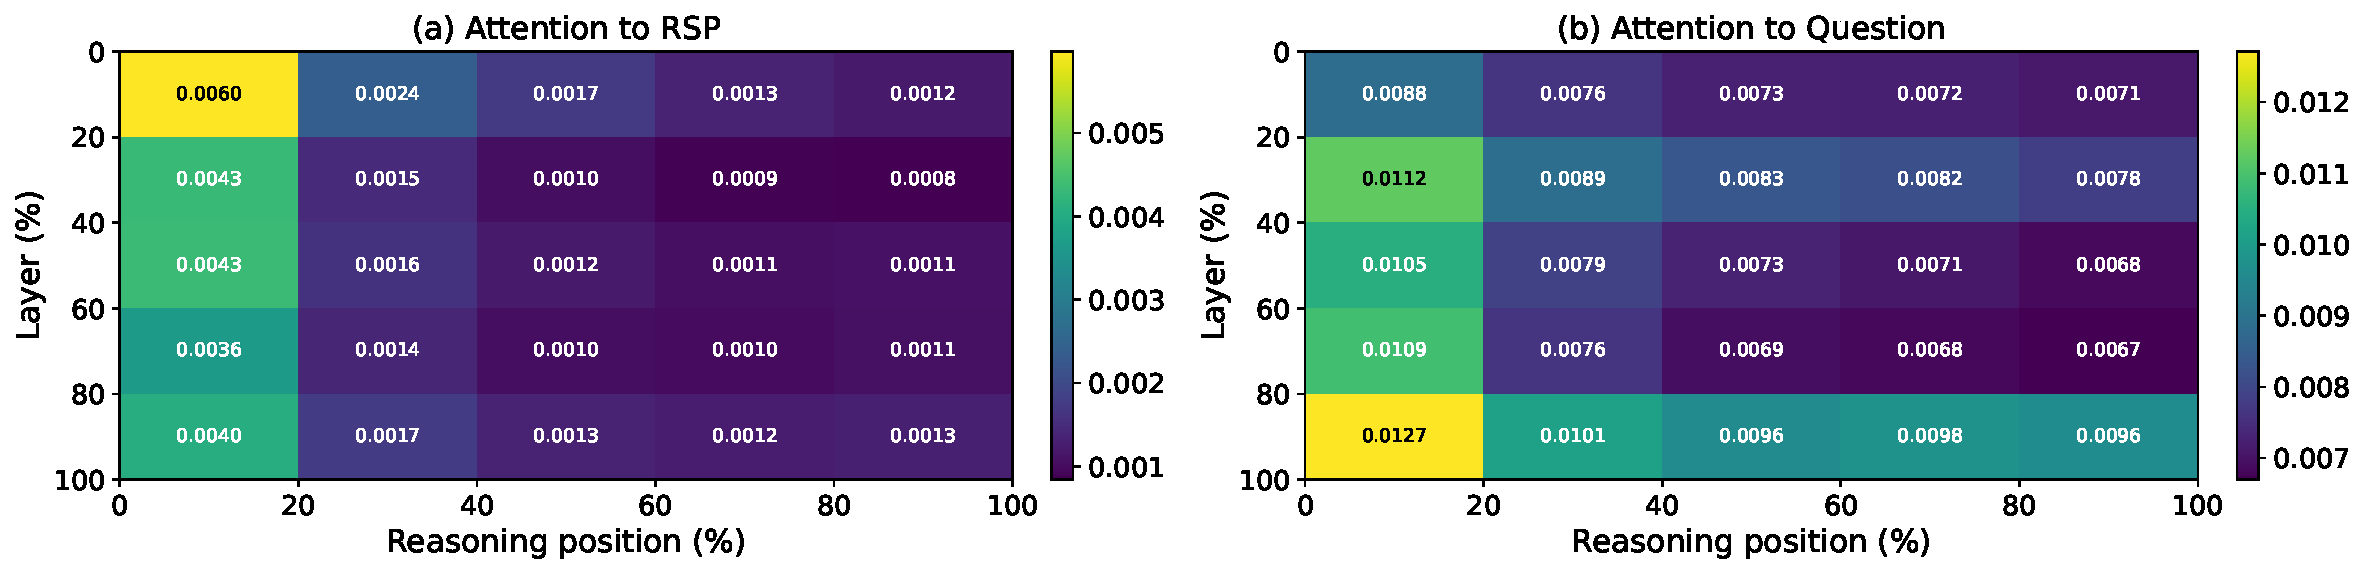
\includegraphics[width=\textwidth]{img/attention/heatmap_qwen1.5b_suffix.pdf}
    \caption{Qwen2.5-Math-1.5B-Instruct, suffix}
  \end{subfigure}
  \\[0.5em]
  \begin{subfigure}[b]{\textwidth}
    \centering
    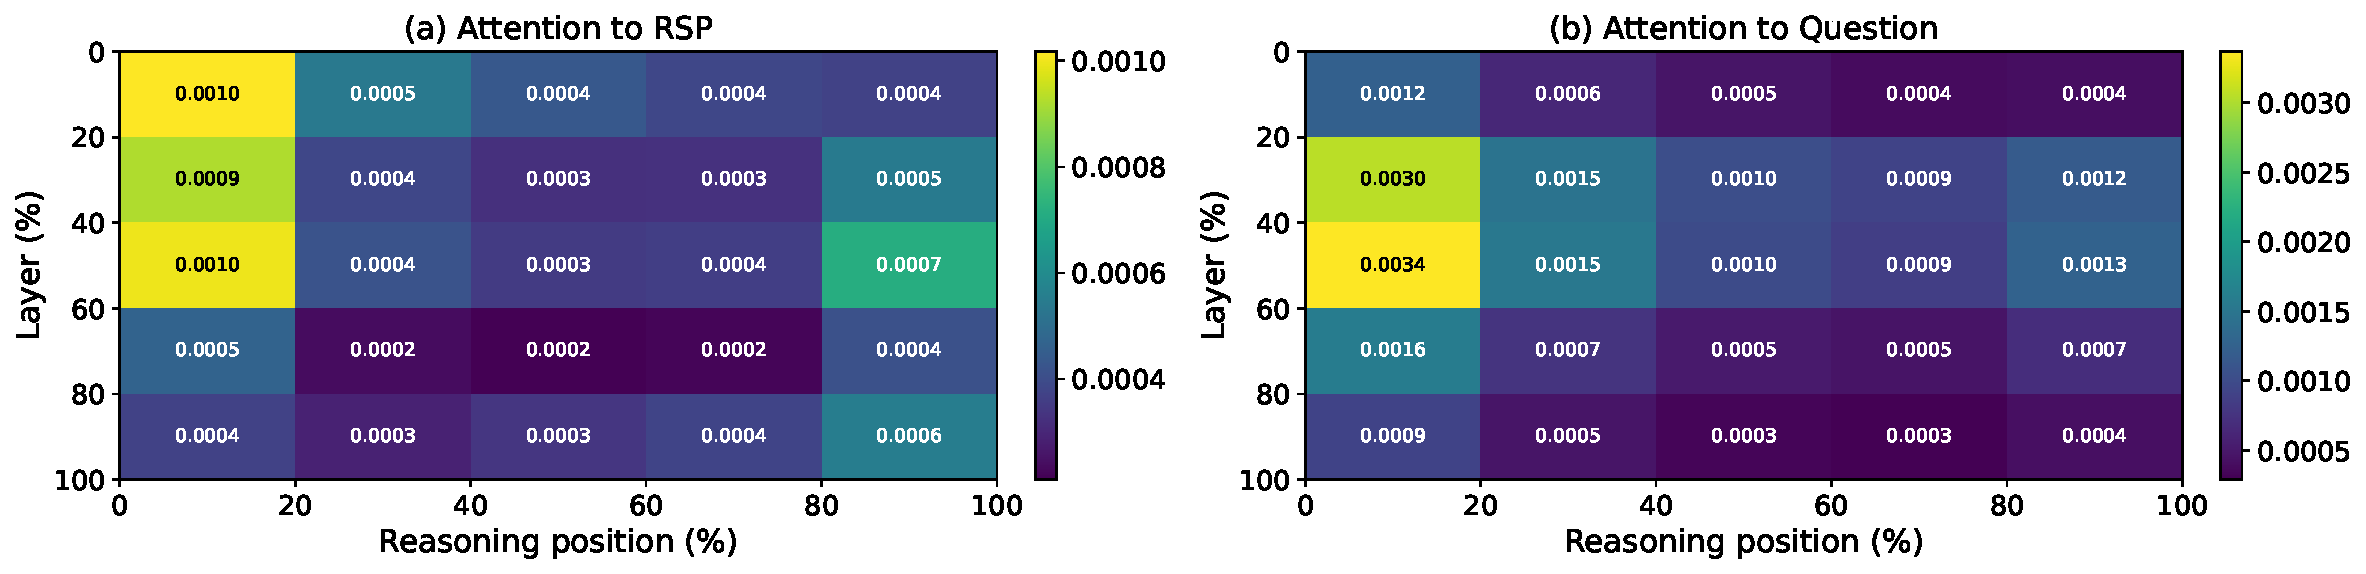
\includegraphics[width=\textwidth]{img/attention/heatmap_llama8b_suffix.pdf}
    \caption{LLaMA-3.1-8B-Instruct, suffix}
  \end{subfigure}
  \caption{나머지 두 모델(각각 500개 MATH-500 샘플)에서 suffix 주입 시 측정한 per-token RSP attention mass. 축과 전처리는 Figure~\ref{fig:attention_mass}와 동일하다. x축은 다섯 분위로 나눈 reasoning position, y축은 다섯 분위로 나눈 layer depth(위가 얕은 층), 색은 RSP 토큰에 할당된 per-token attention의 500샘플 평균을 뜻한다. \texttt{\textbackslash boxed\{\}} 구간 내부 토큰과 마지막 두 레이어는 제외했다.}
  \label{fig:app_attention_additional}
\end{figure}

\clearpage
% ================================================================
\section{GRPO 정식화}\label{app:grpo}
% ================================================================

주어진 프롬프트 $q$에 대해, behavior policy $\pi_{\theta_{\text{old}}}$는 보상 $\{R_i\}_{i=1}^G$를 갖는 응답 집합 $\{o_i\}_{i=1}^G$를 샘플링한다. 각 응답의 advantage는 그룹 수준 보상을 정규화해 계산한다.
\begin{equation}
  \hat{A}_{i,t} = \frac{R_i - \text{mean}(\{R_i\}_{i=1}^G)}{\text{std}(\{R_i\}_{i=1}^G)}.
\end{equation}
정책은 KL penalty가 포함된 clipped objective로 업데이트한다.
\begin{equation}
  \mathcal{J}_{\text{GRPO}}(\theta) = \mathbb{E} \left[ \frac{1}{G} \sum_{i=1}^{G} \frac{1}{|o_i|} \sum_{t=1}^{|o_i|} \left( \min\left( r_{i,t} \hat{A}_{i,t},\; \text{clip}(r_{i,t}, 1\!-\!\varepsilon, 1\!+\!\varepsilon)\, \hat{A}_{i,t} \right) - \beta D_{\text{KL}}(\pi_\theta \| \pi_{\text{ref}}) \right) \right],
\end{equation}
여기서 $r_{i,t} = \pi_\theta(o_{i,t} \mid q, o_{i,<t}) / \pi_{\theta_{\text{old}}}(o_{i,t} \mid q, o_{i,<t})$는 importance sampling ratio이고, $\varepsilon$는 clipping 범위, $\beta$는 reference policy $\pi_{\text{ref}}$에 대한 KL penalty 세기를 조절한다.

\clearpage
% ================================================================
\section{광범위한 영향}\label{app:broader_impacts}
% ================================================================

본 연구는 무작위 임베딩 주입이 대형 언어 모델의 추론 행동에 어떤 영향을 주는지에 대한 실험적·이론적 분석을 제공한다. 기여의 성격은 주로 기초 연구에 가깝지만, GRPO와 같은 강화학습 기반 추론 모델 후속학습에는 잠재적 함의를 가진다.

\paragraph{긍정적 영향.}
RSP가 유도하는 궤적 다양성은 group-relative advantage estimation 안에서 더 풍부한 학습 신호를 제공함으로써, RL 기반 LLM 후속학습의 sample efficiency를 높일 수 있다. 이는 reasoning 중심 fine-tuning과 alignment에 필요한 계산 비용을 줄여, 자원이 제한된 연구 그룹에도 관련 방법을 더 접근 가능하게 만들 수 있다.

\paragraph{잠재적 우려.}
LLM의 유효 출력 지지 집합을 넓히는 방법은 바람직한 대안적 추론 경로뿐 아니라, 바람직하지 않거나 분포 밖에 있는 출력의 도달 가능성도 함께 높일 수 있다. 따라서 RSP를 실제 시스템에 적용할 때는 이를 독립적인 다양성 원천으로만 보지 말고, 기존의 안전 필터링 및 alignment 메커니즘과 함께 사용해야 한다.

\paragraph{영향 범위의 한계.}
본 연구는 새로운 모델이나 데이터셋을 배포하기보다 분석을 제공하는 데 초점을 두므로, 직접적인 사회적 영향은 제한적이다. 여기서 논의한 더 넓은 함의는 RSP가 실제 학습 파이프라인에 통합되는 향후 연구가 이루어질 때에만 현실화될 수 있다.
